\documentclass{article}

% Formatting
\usepackage[utf8]{inputenc}
\usepackage[margin=1in]{geometry}
\usepackage[titletoc,title]{appendix}
\usepackage{graphicx}
\usepackage{breqn}
\usepackage{amsmath}
\usepackage{multirow}
\usepackage{float}


\graphicspath{ {/Volumes/timothyelder/Graduate/Maximum_Likelihood/assessment_final/figures/} }

% Title content
\title{The Prevalence and Predictors of Advance Care Directives for Home Health Care Patients}
\author{Timothy Elder}
\date{December 10th, 2020}

\begin{document}

\maketitle

% Introduction and Overview
\section{Introduction}

Advance care directives are a means for individuals to plan for the healthcare they want to receive if they experience a medical crisis. This includes the type of care and the extent of care they will receive if they are to become incapacitated or rendered legally incompetent, particularly in circumstances where their illness is acute and life threatening. In conjunction with more specific provisions for medical decision making, such as designating a medical proxy or representative with durable power of attorney, they represent the principle means by which individuals can plan for the future when they become ill with life limiting and terminal illnesses. 

The importance of Advance Directives are heightened in the contemporary landscape of illness and death, where death is an "expected and protracted process" \cite{carr_well-being_2019} and medical protocols persist in maintaining life sustaining therapies as the default procedure \cite{timmermans_sudden_1999}. Advance directives are a means for regulating the kind of end of life care individuals will receive in advance of their death, a process that is fraught with a variety of decisions with consequential results for patient and family well-being, both in the terminal phase of illness, but in the case of family members, the impacts extend into bereavement. 

Of note are a variety of gaps in the utilization of these directives in advance of death, particularly by racial minorities and for low income individuals \cite{carr_advance_2017, laguna_jeff_racialethnic_2014}. Further, there is equivocal evidence regarding the efficacy of these directives to really shape the kind of care that patients receive and the quality of life they have at the end of life. 

% Model 
\section{Data and Methods}

The National Hospice and Home Health Care Study (2007) is a national representative sample of U.S. home health and hospice agencies. The data was collected by sampling home health and hospice agencies and used the agency's administrative records to collect patient level measures of a variety consequential attributes for the care of those experiencing life limiting illnesses. The data consists of 1,036 agencies and 9,416 home health (N = 4683) and hospice discharges (N = 4733). These populations warrant different analyses as they are fundamentally different types. The hospice discharges include both current and former patients, discharged from hospice care for a variety of reasons including death. The home health patients are those individuals receiving home health services in the home provided by an agency. For the analyses below I focus on the current home health patients as the social context of interest here is acutely ill individuals who are not already undergoing explicitly \emph{palliative} therapies. By definition, to receive hospice care in the US, one has to have a prognosis of 6 or fewer months. Analyzing home health patients allows me to examine patients with a variety of prognoses, including he terminally ill, and see to what degree a terminal diagnosis might influence the utilization of Advance Directives, which as explained above, are considered integral to specifying end of life care. 

The model is a powerful tool for understanding the condition of patients in these healthcare contexts, including their symptom load, the use of services including social services, as well as the place of death and the kind of advance care planning that is the focus of the current manuscript. The analyses undertaken here do not take full advantage of the survey design and specifically the survey weights which allow for the inference from the sample to national representation \cite{laguna_jeff_racialethnic_2014}. The handling of survey weights will be elaborated upon more fully below, but suffice to say that I have compared the model using and not using survey weights and diagnostics indicate the differences are marginal in terms of precision, effect size and direction. 

The analyses below are meant to capture several features of patients that are likely to influence the propensity to utilize advance directives, as well as typical scenarios in which advance directives are generally taken to be an integral part of managing their care. The focal characteristics are symptom profile or symptom burden, attributes such as being embedded in social relations, socioeconomic status, and several controls including duration of current care episode. Variables of interest, the attribute they are meant to capture, and a description are given in Table 1. 

\begin{table}[h]
\begin{tabular}{ccl}
\multicolumn{1}{c|}{Attribute of Interest} &
  \multicolumn{1}{c|}{Variable} &
  \multicolumn{1}{c}{Description} \\ \hline
\multirow{4}{*}{\begin{tabular}[c]{@{}c@{}}Symptom Profile/ \\ Symptom Burden\end{tabular}} &
  TOTPROC &
  Total number of procedures the patient has had \\
                           & TOTCDDX  & Total number of primary diagnoses the patient has             \\
                           & TOTALRX  & Total number of prescription drugs patient is prescribed      \\
                           & COGNFUNC & Cognitive function (1 = No Impairment, 5 = Severely Impaired) \\ \hline
\multirow{2}{*}{Prognosis} & TERMINAL & 6 months or less prognosis (0,1)                              \\
                           & READMSS  & Readmission to home health care (0,1)                         \\ \hline
Socioeconomic Status       & MCAIDENR & Enrolled in Medicaid (0,1)                                    \\ \hline
Social Profile             & MARRIED  & Married (0,1)                                                 \\ \hline
\multirow{3}{*}{Controls}  & LOSHH    & Length of current episode of care (Log)                            \\
                           & AGEATINT & Current age of patient at time of interview                   \\
                           & SEX      & Male = 1, Female = 0                                         
\end{tabular}
\caption{Independent variables and patient attributes of interest.}
\end{table}

\begin{table}[h]\centering 
\begin{tabular}{lllllll}
Statistic &
  \multicolumn{1}{c}{Mean} &
  \multicolumn{1}{c}{St. Dev.} &
  \multicolumn{1}{c}{Min} &
  \multicolumn{1}{c}{Pctl(25)} &
  \multicolumn{1}{c}{Pctl(75)} &
  \multicolumn{1}{c}{Max} \\ \hline
ANYADDIR   & 0.321   & 0.467   & 0     & 0     & 1     & 1     \\
SEX        & 0.375   & 0.484   & 0     & 0     & 1     & 1     \\
AGEATINT   & 68.519  & 21.949  & 0     & 60    & 84    & 100   \\
MARRIED    & 0.368   & 0.482   & 0     & 0     & 1     & 1     \\
TERMINAL   & 0.149   & 0.356   & 0     & 0     & 0     & 1     \\
log\_LOSHH & 4.520   & 1.538   & 0.693 & 3.332 & 5.823 & 6.999 \\
LOSHH      & 249.814 & 336.212 & 1     & 27    & 337   & 1,095 \\
READMSS    & 0.303   & 0.460   & 0     & 0     & 1     & 1     \\
TOTCDDX    & 4.402   & 2.369   & 0     & 3     & 6     & 16    \\
TOTALRX    & 10.740  & 5.543   & 0     & 7     & 14    & 25    \\
TOTPROC    & 0.361   & 0.661   & 0     & 0     & 1     & 5     \\
MCAIDENR   & 0.352   & 0.478   & 0     & 0     & 1     & 1     \\
HISPAN     & 0.061   & 0.239   & 0     & 0     & 0     & 1     \\
RACEWHT    & 0.869   & 0.338   & 0     & 1     & 1     & 1     \\
RACEBLCK   & 0.110   & 0.313   & 0     & 0     & 0     & 1    
\end{tabular}
\caption{Descriptive statistics for variables of interest.}
\end{table}

The variable for length of current care episode was logarithmically transformed, due to the large right skew ($\gamma = 1.56$) as seen in the histograms of IVs in Figure 1. Figure 2 displays a correlation matrix of the Dependent and Independent variables. Note the moderate correlation between the age predictor and the symptom profile measures (except number of procedures), as well as the negative correlation between length of stay and being a medicaid enrollee. Further note lack of strong collinearity between the IVs. 

The NHHCS data includes a complex survey design and sample weights. Due to the lack of \texttt{R} packages for survey data which use maximum likelihood estimation for logistic regression I have opted to exclude survey weights in my analysis. This undermines the ability to generalize the findings to a larger population. Table 2 displays coefficients and standard errors from a weighted and unweighted model, and there do not seem to be obvious and substantive differences in effect size, direction, or standard errors when between the weighted and unweighted models.

% Hypotheses
\section{Hypotheses}

\textbf{Hypothesis \#1} : Hypothesis 1 relates to the features of patients which relate to symptom burden and prognosis, with all the variables in these two categories (indicated above) to increase the probability of having an advance directive. This is likely as the variables indicate worsening illnesses, shorter prognoses, and generally Indicate that an individual is approaching the end of life. The variable for cognitive function is likely to have a powerful effect, as individuals experiencing diminished cognitive capacities will likely have had an earlier opportunity to create a plan fo their care in advance of losing their faculties. 

\textbf{Hypothesis \#2}: Being married is likely to also increase the probability of having an advance directive. Advance directives are not only a means of planning for care, but has the further effect of mediating burden on relatives who are the default decision makers for a patient who is no longer able to make decisions for themselves. Qualitative research on terminally ill patients has found that one of the most distressing psycho-social stressors in the end of life, is the fear of being a burden and undermining family members well-being by leaving them with the burden of decision making {oxford textbook}. 

\textbf{Hypothesis \#3}: Medicaid enrollees are less likely to have advance directives, as they have fewer opportunities to be exposed to information related to their use and implementation. This is in part due to the fact that lower SES individuals have more infrequent interactions with health care professionals, even in the context of life limiting illness. \cite{carr_is_2016}


% Results
\section{Results}

Logistic regression results are displayed in Table 3. Model 2 seems to support Hypotheses 1 and 3. Curiously, the MARRIED indicator variable runs in the opposite direction as hypothesized. Calculating first differences for a few of the focal variables leads to equivocal results regarding the model coefficients. The base proportion of home healthcare patients in the dataset with an advance directive is 30\%. The estimated probability of a terminally ill women, who was not readmitted to care, with mean cognitive function, mean age and mean length of stay in care is 98\%, while a patient under the same conditions who is not terminally ill has a 97\% probability of having an advance directive. 

Plotting some of these scenarios further complicates the findings. Line graphs displaying the probability of having an advance directive in various scenarios of interest are displayed in Figure 4. The differences between men and women are nominal, as well as for married and unmarried individuals. Differences in the probability of having an advance directive between terminally ill and non-terminally ill patients is not able at older ages, while the probability for medicaid enrollees is consistently lower than non-enrolled patients. This is the opposite relationship as reported in Table 3, and what more, the probabilities in the visualizations never arise to the levels reported n the calculations of first differences. 

\begin{table}[h] \centering 
  \caption{Coefficients and Standard Errors for null, base and full model.} 
  \label{} 
\begin{tabular}{@{\extracolsep{5pt}}lccc} 
\\[-1.8ex]\hline 
\hline \\[-1.8ex] 
 & \multicolumn{3}{c}{\textit{Dependent variable:}} \\ 
\cline{2-4} 
\\[-1.8ex] & \multicolumn{3}{c}{ANYADDIR} \\ 
\\[-1.8ex] & (1) & (2) & (3)\\ 
\hline \\[-1.8ex] 
 SEX &  & $-$0.070 & $-$0.079 \\ 
  &  & (0.079) & (0.080) \\ 
  & & & \\ 
 AGEATINT &  & 0.023$^{***}$ & 0.023$^{***}$ \\ 
  &  & (0.002) & (0.002) \\ 
  & & & \\ 
 COGNFUNC &  & 0.089$^{**}$ & 0.107$^{***}$ \\ 
  &  & (0.035) & (0.035) \\ 
  & & & \\ 
 MARRIED &  & $-$0.072 & $-$0.084 \\ 
  &  & (0.080) & (0.082) \\ 
  & & & \\ 
 TERMINAL &  & 0.298$^{***}$ & 0.257$^{***}$ \\ 
  &  & (0.098) & (0.100) \\ 
  & & & \\ 
 log\_LOSHH &  & $-$0.013 & $-$0.004 \\ 
  &  & (0.026) & (0.027) \\ 
  & & & \\ 
 READMSS &  & 0.032 & 0.016 \\ 
  &  & (0.080) & (0.081) \\ 
  & & & \\ 
 TOTCDDX &  & 0.042$^{**}$ & 0.040$^{**}$ \\ 
  &  & (0.017) & (0.017) \\ 
  & & & \\ 
 TOTALRX &  & 0.029$^{***}$ & 0.022$^{***}$ \\ 
  &  & (0.007) & (0.007) \\ 
  & & & \\ 
 TOTPROC &  & 0.149$^{**}$ & 0.133$^{**}$ \\ 
  &  & (0.058) & (0.059) \\ 
  & & & \\ 
 MCAIDENR &  & $-$0.499$^{***}$ & $-$0.376$^{***}$ \\ 
  &  & (0.092) & (0.094) \\ 
  & & & \\ 
 HISPAN &  &  & $-$1.001$^{***}$ \\ 
  &  &  & (0.196) \\ 
  & & & \\ 
 RACEBLCK &  &  & $-$0.165 \\ 
  &  &  & (0.359) \\ 
  & & & \\ 
 RACEWHT &  &  & 1.066$^{***}$ \\ 
  &  &  & (0.329) \\ 
  & & & \\ 
 Constant & $-$0.750$^{***}$ & $-$2.817$^{***}$ & $-$3.717$^{***}$ \\ 
  & (0.035) & (0.232) & (0.399) \\ 
  & & & \\ 
\hline \\[-1.8ex] 
Observations & 3,783 & 3,783 & 3,783 \\ 
Log Likelihood & $-$2,374.033 & $-$2,214.199 & $-$2,158.504 \\ 
Akaike Inf. Crit. & 4,750.066 & 4,452.399 & 4,347.007 \\ 
\hline 
\hline \\[-1.8ex] 
\textit{Note:}  & \multicolumn{3}{r}{$^{*}$p$<$0.1; $^{**}$p$<$0.05; $^{***}$p$<$0.01} \\ 
\end{tabular} 
\end{table} 

% Discussion
\section{Discussion}

The results of the logistic regression are ambiguous. Making any conclusions regarding the veracity of the hypotheses would be premature. The ambiguity is a result of varied results between the BUTON of the model, the calculation of first differences, and the vizualization of the probabilities in focal scenarios across patients ages. 

This may be in part due to the models' quality. The ROC plot for the model in Figure 6 below, shows that the model is marginally better than chance in predicting the true value of the dependent variable. Table 4 displays the predicted vs. the observed values for the dependent variable with a 68\% rate of success. The log-likelihood of the full model is lower than the null model (Full Model $\ell = -2213.718 $, Null Model $\ell = -2374.033 $ ), though the BIC for the null vs. the full model is comparatively better (Full Model BIC = 4526.29, Null Model BIC = 4756.304). 

\begin{table}[h]
\centering
\begin{tabular}{rrr}
  \hline
 & Observed 0 & Observed 1 \\ 
  \hline
Predicted 0 & 2456 & 1039 \\ 
  Predicted 1 & 113 & 175 \\ 
   \hline
\end{tabular}
\caption{Predicted at c=.5 or greater.} 
\end{table}


% Bibliography

\bibliographystyle{apa}
\bibliography{/Volumes/timothyelder/Graduate/Maximum_Likelihood/assessment_final/tex_assessment_final/bibliography}

% Appendix
\section{Appendix A: Supplemental Figures}
\begin{appendix}

\begin{figure}[h]
\centering
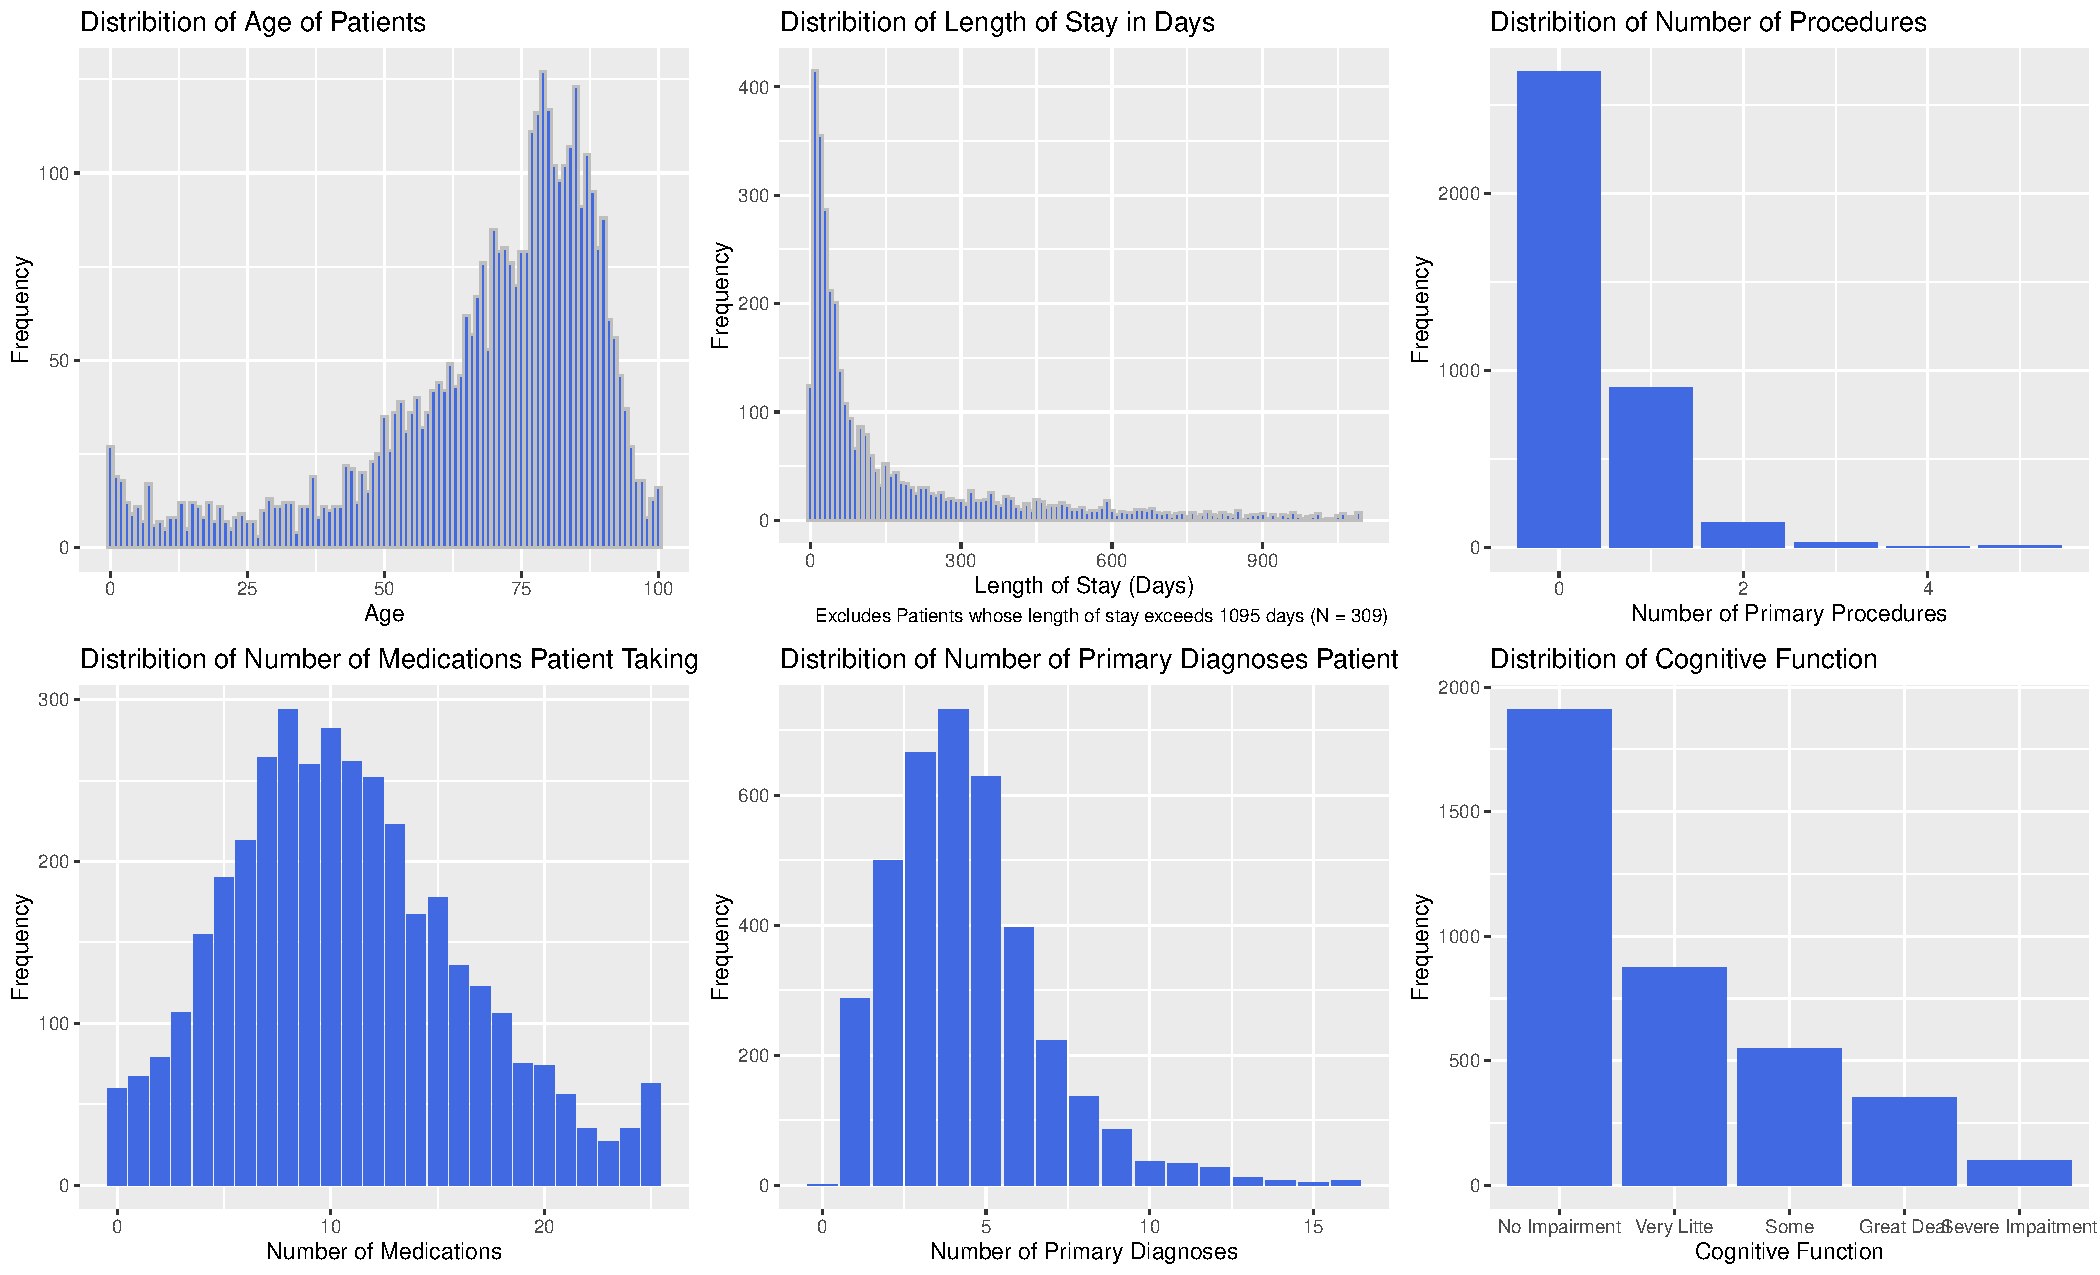
\includegraphics[width=15cm]{distributions_ivs}
\caption{Distributions of Independent Variables.}
\end{figure}

\begin{figure}[h]
\centering
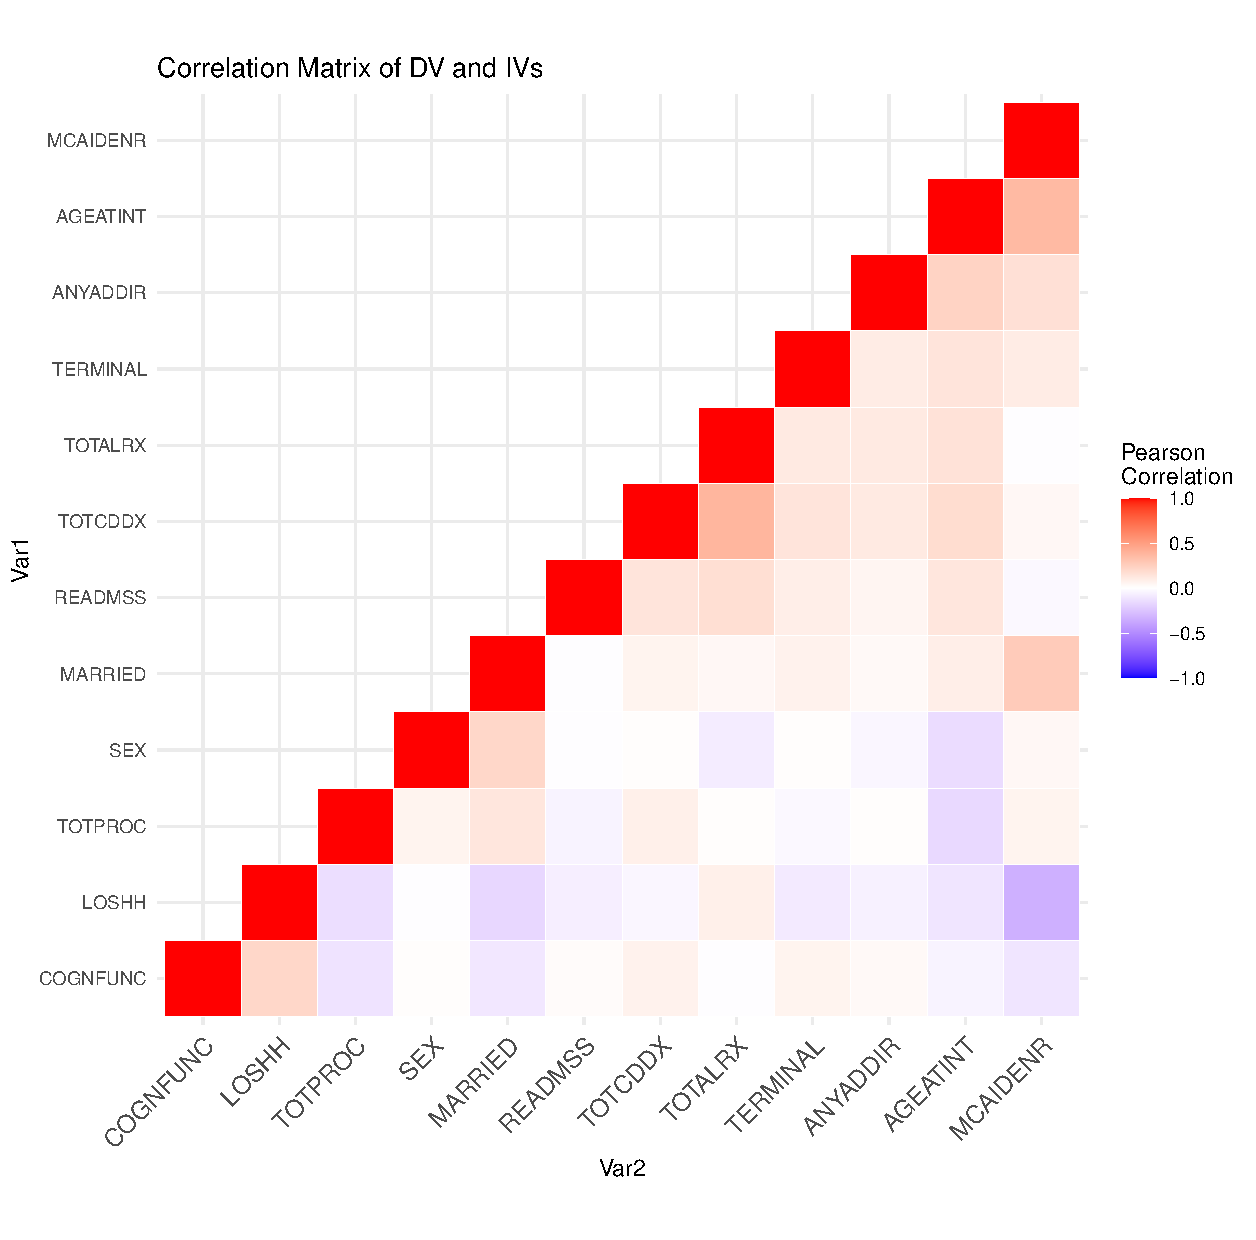
\includegraphics[width=10cm]{cor_heatmap}
\caption{Correlation Matrix of Dependent Variable and Predictors.}
\end{figure}

\begin{figure}[h]
\centering
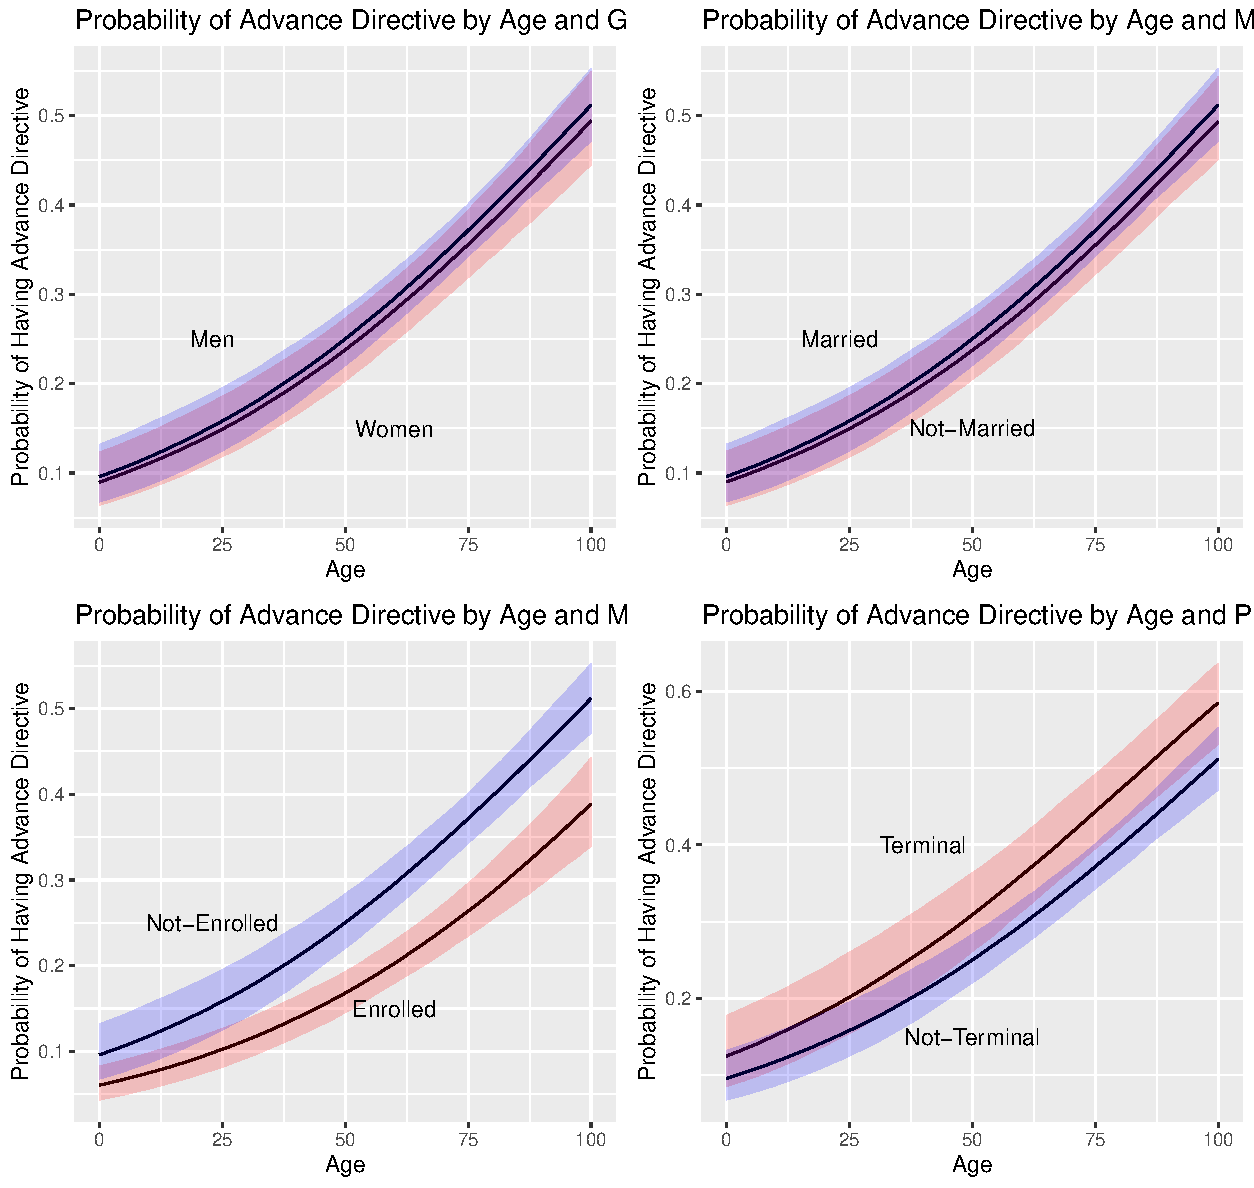
\includegraphics[width=15cm]{all_lines}
\caption{Probabilities of Advance Directive under various scenarios. Unless otherwise specified each graph is for female, unmarried patients, not enrolled in medicaid, who are not terminally ill.}
\end{figure}

\section{Appendix B: Model Diagnostics}

\begin{table}[h] \centering 
  \caption{Coefficients and standard errors comparing the unweighted and survey weighted logistic regression results.} 
  \label{} 
\begin{tabular}{@{\extracolsep{5pt}}lcc} 
\\[-1.8ex]\hline 
\hline \\[-1.8ex] 
 & \multicolumn{2}{c}{\textit{Dependent variable:}} \\ 
\cline{2-3} 
\\[-1.8ex] & \multicolumn{2}{c}{ANYADDIR} \\ 
\\[-1.8ex] & \textit{logistic} & \textit{survey-weighted} \\ 
 & \textit{} & \textit{logistic} \\ 
\\[-1.8ex] & (1) & (2)\\ 
\hline \\[-1.8ex] 
 SEX & $-$0.070 & $-$0.054 \\ 
  & (0.079) & (0.143) \\ 
  & & \\ 
 AGEATINT & 0.023$^{***}$ & 0.019$^{***}$ \\ 
  & (0.002) & (0.004) \\ 
  & & \\ 
 COGNFUNC & 0.092$^{***}$ & 0.071 \\ 
  & (0.035) & (0.062) \\ 
  & & \\ 
 MARRIED & $-$0.075 & $-$0.109 \\ 
  & (0.080) & (0.142) \\ 
  & & \\ 
 TERMINAL & 0.292$^{***}$ & 0.242 \\ 
  & (0.098) & (0.179) \\ 
  & & \\ 
 LOSHH & $-$0.0001 & $-$0.0001 \\ 
  & (0.0001) & (0.0002) \\ 
  & & \\ 
 READMSS & 0.024 & 0.139 \\ 
  & (0.080) & (0.147) \\ 
  & & \\ 
 TOTCDDX & 0.042$^{**}$ & 0.009 \\ 
  & (0.017) & (0.032) \\ 
  & & \\ 
 TOTALRX & 0.029$^{***}$ & 0.031$^{**}$ \\ 
  & (0.007) & (0.013) \\ 
  & & \\ 
 TOTPROC & 0.146$^{**}$ & 0.178 \\ 
  & (0.058) & (0.114) \\ 
  & & \\ 
 MCAIDENR & $-$0.484$^{***}$ & $-$0.812$^{***}$ \\ 
  & (0.092) & (0.160) \\ 
  & & \\ 
 Constant & $-$2.849$^{***}$ & $-$2.427$^{***}$ \\ 
  & (0.211) & (0.338) \\ 
  & & \\ 
\hline \\[-1.8ex] 
Observations & 3,783 & 3,783 \\ 
Log Likelihood & $-$2,213.718 & $-$2,006.713 \\ 
Akaike Inf. Crit. & 4,451.435 & 4,037.427 \\ 
\hline 
\hline \\[-1.8ex] 
\textit{Note:}  & \multicolumn{2}{r}{$^{*}$p$<$0.1; $^{**}$p$<$0.05; $^{***}$p$<$0.01} \\ 
\end{tabular} 
\end{table} 

\begin{figure}[h]
\centering
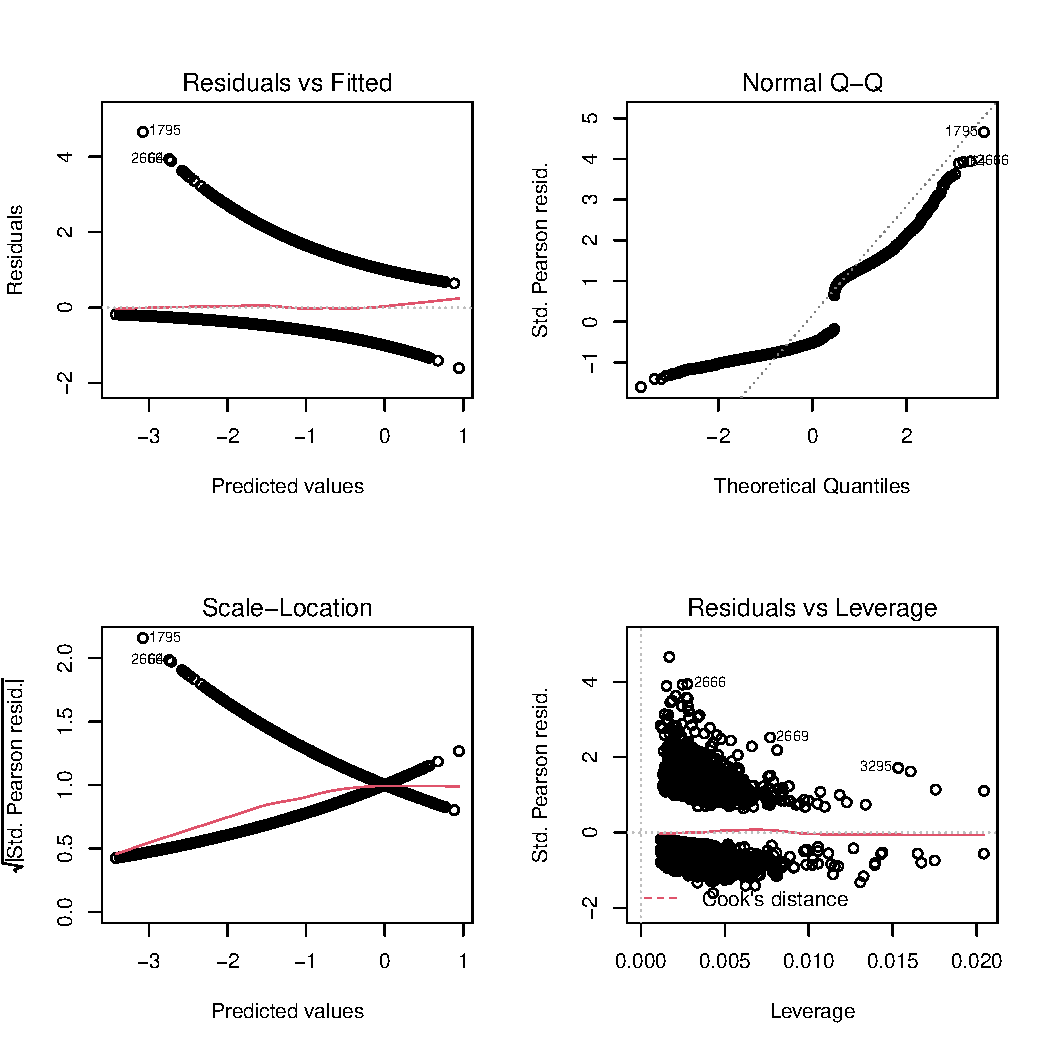
\includegraphics[width=7cm]{unweighted_dir_logit_modelfit_base}
\caption{Base Plot of Model Diagnostics.}
\end{figure}

\begin{figure}[h]
\centering
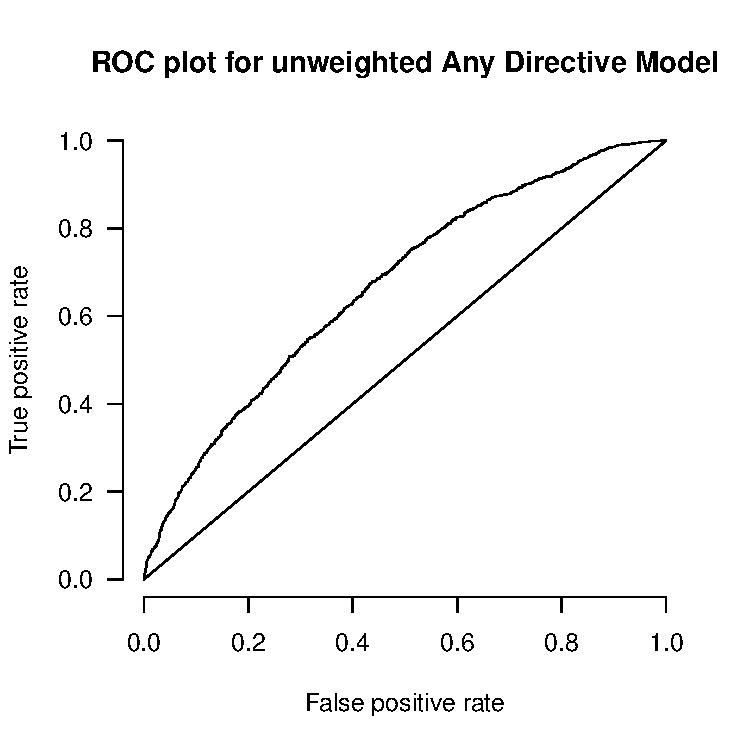
\includegraphics[width=7cm]{anydirective_unweighted_ROC}
\caption{ROC plot for Model.}
\end{figure}

\end{appendix}

\end{document}
